\subsection{Experiment Setup} \label{Experiment_Setup}

The experiment consists of the AAC subsystem, with six sampling bags, and the CAC coiled tube subsystem. Shown in Figure {\ref{fig:3D_tubular_render}}, the CAC is fitted into the partition on the left, and the AAC into the partition to the right. The principal aim is to validate the AAC sampling method. To do so, it is necessary to sample during Descent Phase in order to compare the results with the ones obtained from the CAC. This is because the CAC collects its air sample passively by pressure differentials in the descent. Flight speeds mentioned in this section have been obtained from the BEXUS manual as well as through analysis of past flights. Figure \ref{fig:block-diagram} shows a generic block diagram of the main subsystems interconnection.

\begin{figure}[H]
    \begin{align*}
        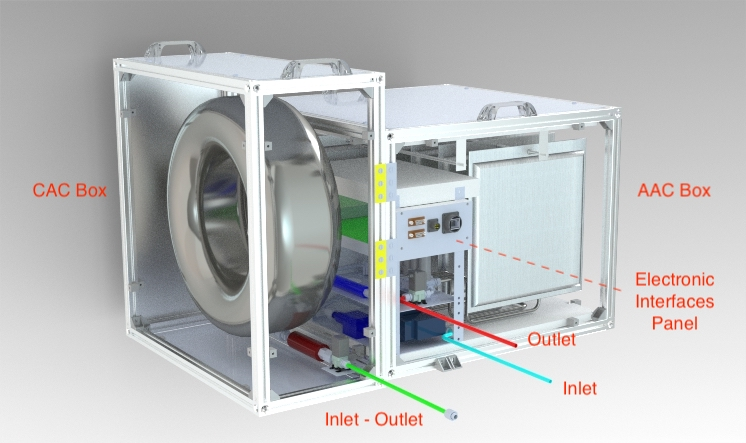
\includegraphics[width=1\linewidth]{4-experiment-design/img/Mechanical/v9_3D.jpg}
    \end{align*}
    \caption{Physical Setup of the Experiment.}
    \label{fig:3D_tubular_render}
\end{figure}

\begin{figure}[H]
    \begin{align*}
        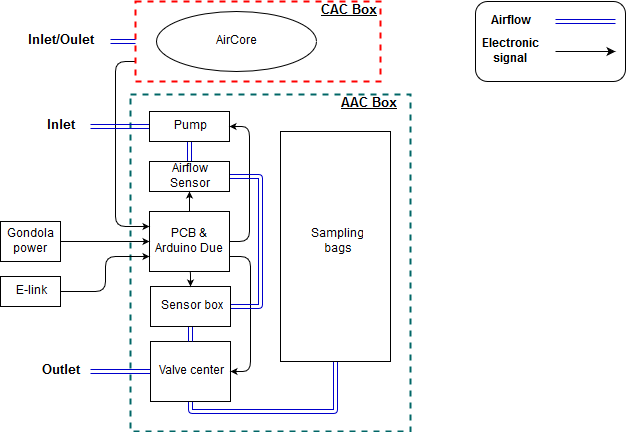
\includegraphics[width=1\linewidth]{4-experiment-design/img/Mechanical/Block-Diagram.png}
    \end{align*}
    \caption{Block Diagram of the Experiment.}
    \label{fig:block-diagram}
\end{figure}

The primary concern regarding the AAC air sampling subsystem occurs after the cut-off when the gondola will tumble and fall at an average speed of 50 m/s for approximately two minutes \cite{BexusManual}. This descent speed is too large in order to sample air at the desired vertical resolution, capped at 500 m. As such, sampling can only be done after the gondola has stabilized at a descent speed  of 8 m/s \cite{BexusManual}. The tumbling phase will vertically span for approximately 6 km. Considering a Float Phase altitude of 25 km, sampling during the Descent Phase will commence at approximately 19 km in altitude. However, the primary region of interest in terms of sampling is in the stratosphere, particularly between 19 km and 25 km in altitude. Sampling will thus also occur during the Ascent Phase. Out of the six sampling bags present in the payload, two will be used during the Ascent Phase at 18 km and 21 km and four during the Descent Phase at 17.5 km, 16 km, 14 km and 12 km as seen in Table \ref{tab:sampling-altitudes}. Details regarding the sampling strategy can be found in Appendix \ref{sec:appH}.

\begin{table}[H]
\centering
\begin{tabular}{|c|c|c|c|}
\hline
\multicolumn{1}{|l|}{} & \multicolumn{1}{l|}{\textbf{Sampling Altitudes}} & \multicolumn{1}{l|}{\textbf{Ambient Pressure}} & \multicolumn{1}{l|}{\textbf{Ambient Temperature}} \\ \hline
\multirow{2}{*}{\textbf{Ascent Phase}} & 18 km & 75.0 hPa & 216.7 K \\ \cline{2-4} 
 & 21 km & 46.8 hPa & 217.6 K \\ \hline
\multirow{4}{*}{\textbf{Descent Phase}} & 17.5 km & 81.2 hPa & 216.7 K \\ \cline{2-4} 
 & 16 km & 102.9 hPa & 216.7 K \\ \cline{2-4} 
 & 14 km & 141.0 hPa & 216.7 K \\ \cline{2-4} 
 & 12 km & 193.3 hPa & 216.7 K \\ \hline
\end{tabular}
\caption{Sampling Altitudes as well as the Corresponding Ambient Pressures and Temperatures According to the 1976 US Standard Atmosphere.}
\label{tab:sampling-altitudes}
\end{table}

The maximum pressure that the sampling bags can withstand has to be taken into account in order to avoid bursting. Decreasing pressure during the Ascent Phase poses a risk to sampling bags which already contain samples as the gas inside will expand which may cause the bag to burst. In order to avoid this, the sampling bags will not be completely filled. Filling up to a maximum of 80\% of the sampling bag's capacity (2 psi/0.14 bar) is recommended by the manufacturers for the Multi-Layer Foil sampling bags that are to be used. The inverse is also true for the Descent Phase where compression will occur. As such, the sampling bags should be fully filled during the Descent Phase in order to ensure that enough samples are collected for analysis. Past research has revealed that the selected sampling bags can withstand pressure difference of 310 hPa at 30 km of altitude, which is equivalent to 0.31 bar \cite{LISA}. A series of tests listed in Table \ref{tab:sampling-system-test} will be conducted in order to confirm the maximum allowable pressure for the bags.


Due to the difference in pressure between sea level and sampling altitudes, the volume of the sample taken will be considerably reduced when it reaches sea level. This shrinking has to be taken into account as the minimum volume that has to be present in the sampling bag at ground level in order to obtain results with the Picarro analyzer. A minimum amount is required for the analyzer to detect concentrations of the targeted trace gases. This minimum amount is 0.18 L at sea level and it has to be specially considered for the samples taken at higher altitudes. The samples taken at lower altitudes will be exposed to smaller changes in pressure, therefore their size will not be critically reduced. Table \ref{tab:minimum-volume} shows the minimum volume of air that needs to be sampled at different altitudes, in order the sample volume left at sea level pressure is at least 0.18L..  

% Depending on the sampling altitude,there is a minimum volume of air that needs to be sampled in order the sample volume left at sea level pressure is at least 0.18 L. A sample volume of 0.18 L corresponds to the minimum amount required for the Picarro analyzer to detect concentrations of the targeted trace gases. 

% Please add the following required packages to your document preamble:
% \usepackage{multirow}
\begin{table}[]
\centering
\begin{tabular}{|l|l|l|l|l|}
\hline
 & \textbf{\begin{tabular}[c]{@{}l@{}}Minimum \\ Sampling Volume\end{tabular}} & \textbf{\begin{tabular}[c]{@{}l@{}}Sampling \\ Altitudes\end{tabular}} & \textbf{\begin{tabular}[c]{@{}l@{}}Ambient \\ Pressure\end{tabular}} & \textbf{\begin{tabular}[c]{@{}l@{}}Ambient \\ Temperature\end{tabular}} \\ \hline
\multirow{2}{*}{\textbf{Ascent Phase}} & 1.8 L & 18 km & 75.0 hPa & 216.7 K \\ \cline{2-5} 
 & 2.4 L & 21 km & 46.8 hPa & 217.6 K \\ \hline
\multirow{4}{*}{\textbf{Descent Phase}} & 1.7 L & 17.5 km & 81.2 hPa & 216.7 K \\ \cline{2-5} 
 & 1.3 L & 16 km & 102.9 hPa & 216.7 K \\ \cline{2-5} 
 & 1.0 L & 14 km & 141.0 hPa & 216.7 K \\ \cline{2-5} 
 & 0.7 L & 12 km & 193.3 hPa & 216.7 K \\ \hline
\end{tabular}
\caption{Minimum Sampling Volume at Each Altitude to Obtain Enough Air to Perform a Proper Analysis (0.18 L at sea level), Appendix \ref{sec:appH}}
\label{tab:minimum-volume}
\end{table}


The AAC will need an air pump for sampling due to low ambient pressure at stratospheric altitudes. The air pump is also needed in order to assure the intake flow rate and obtain a good resolution. An air pump with an intake rate of at least 3 L/min will be used to ensure that the vertical resolution of the sampling air remains under 500 m during the Ascent Phase's ascent speed of 5 m/s and the  Descent Phase's descent speed of 8 m/s. A flushing valve will be used to flush the AAC system before each bag is filled and make sure that each bag will be filled with fresh air from the corresponding altitude. This filling/flushing procedure occurs twice, the first time during the Ascent Phase for the first two sampling bags and the second time during the Descent Phase for the remaining four sampling bags.

Shortly after the launch, the CAC valve will be opened in order to allow the fill gas that is inside the tube to flush, while the AAC valves will be closed until reaching the sampling altitude. Flushing of the CAC tube happens passively through the progressive decrease in air pressure during the balloon's Ascent Phase and it will be emptied by the time it reaches the Float Phase. Filling of the CAC tube also happens passively through the progressive increase in air pressure during the balloon's Descent Phase. The CAC valve will remain open at all time during the Ascent, Float, and Descent phases. The valve will close just before hitting the ground in order to preserve the sample. 

The ambient pressure will be measured by three pressure sensors located outside the experiment box. Only one of them is necessary for AAC and CAC, but using three will provide redundancy. To measure the pressure inside the bag that is currently being filled, three more sensors will be allocated inside the sensors box. To measure the ambient temperature in the CAC, three sensors will be allocated in the CAC box (in the Styrofoam). Temperature inside the coil is assumed to quickly adjust to the ambient temperature inside the CAC box, therefore there will not be differentiation in temperature between the air inside the tube and the air surrounding the tube. For the bags three more temperature sensors will be placed in the bags' box (in the Styrofoam). To control the temperature for the Arduino, the pump and the valves in the Brain, one temperature sensor will be used for each of them. In total, there will be six pressure sensors and nine temperature sensors. 

The sampling of the AAC will be triggered by the pressure reading from the sensors outside the experiment box. When the required pressure is reached, Table \ref{tab:sampling-altitudes} the valve inside the manifold corresponding to the bag that is to be sampled, will open and the sampling will start. The closing of the valve depends on two conditions and it will be triggered when either one of the conditions is true. These conditions are: maximum sampling time or maximum pressure difference between inside/outside the bags. They are determined from past research \cite{LISA}. A first estimation of the maximum sampling time has already been made, from Test 18 shown in Table \ref{tab:pump-low-pressure-test}, but more tests in the future will determine the maximum pressure condition and confirm the maximum sampling times.

The CAC emptying as well as the AAC and CAC sampling sequence is represented in Figures \ref{fig:ascent} and \ref{fig:descent}. It should be kept in mind that the different pressures are what triggers the opening of the valves. 

\begin{figure}[H]
    \begin{align*}
        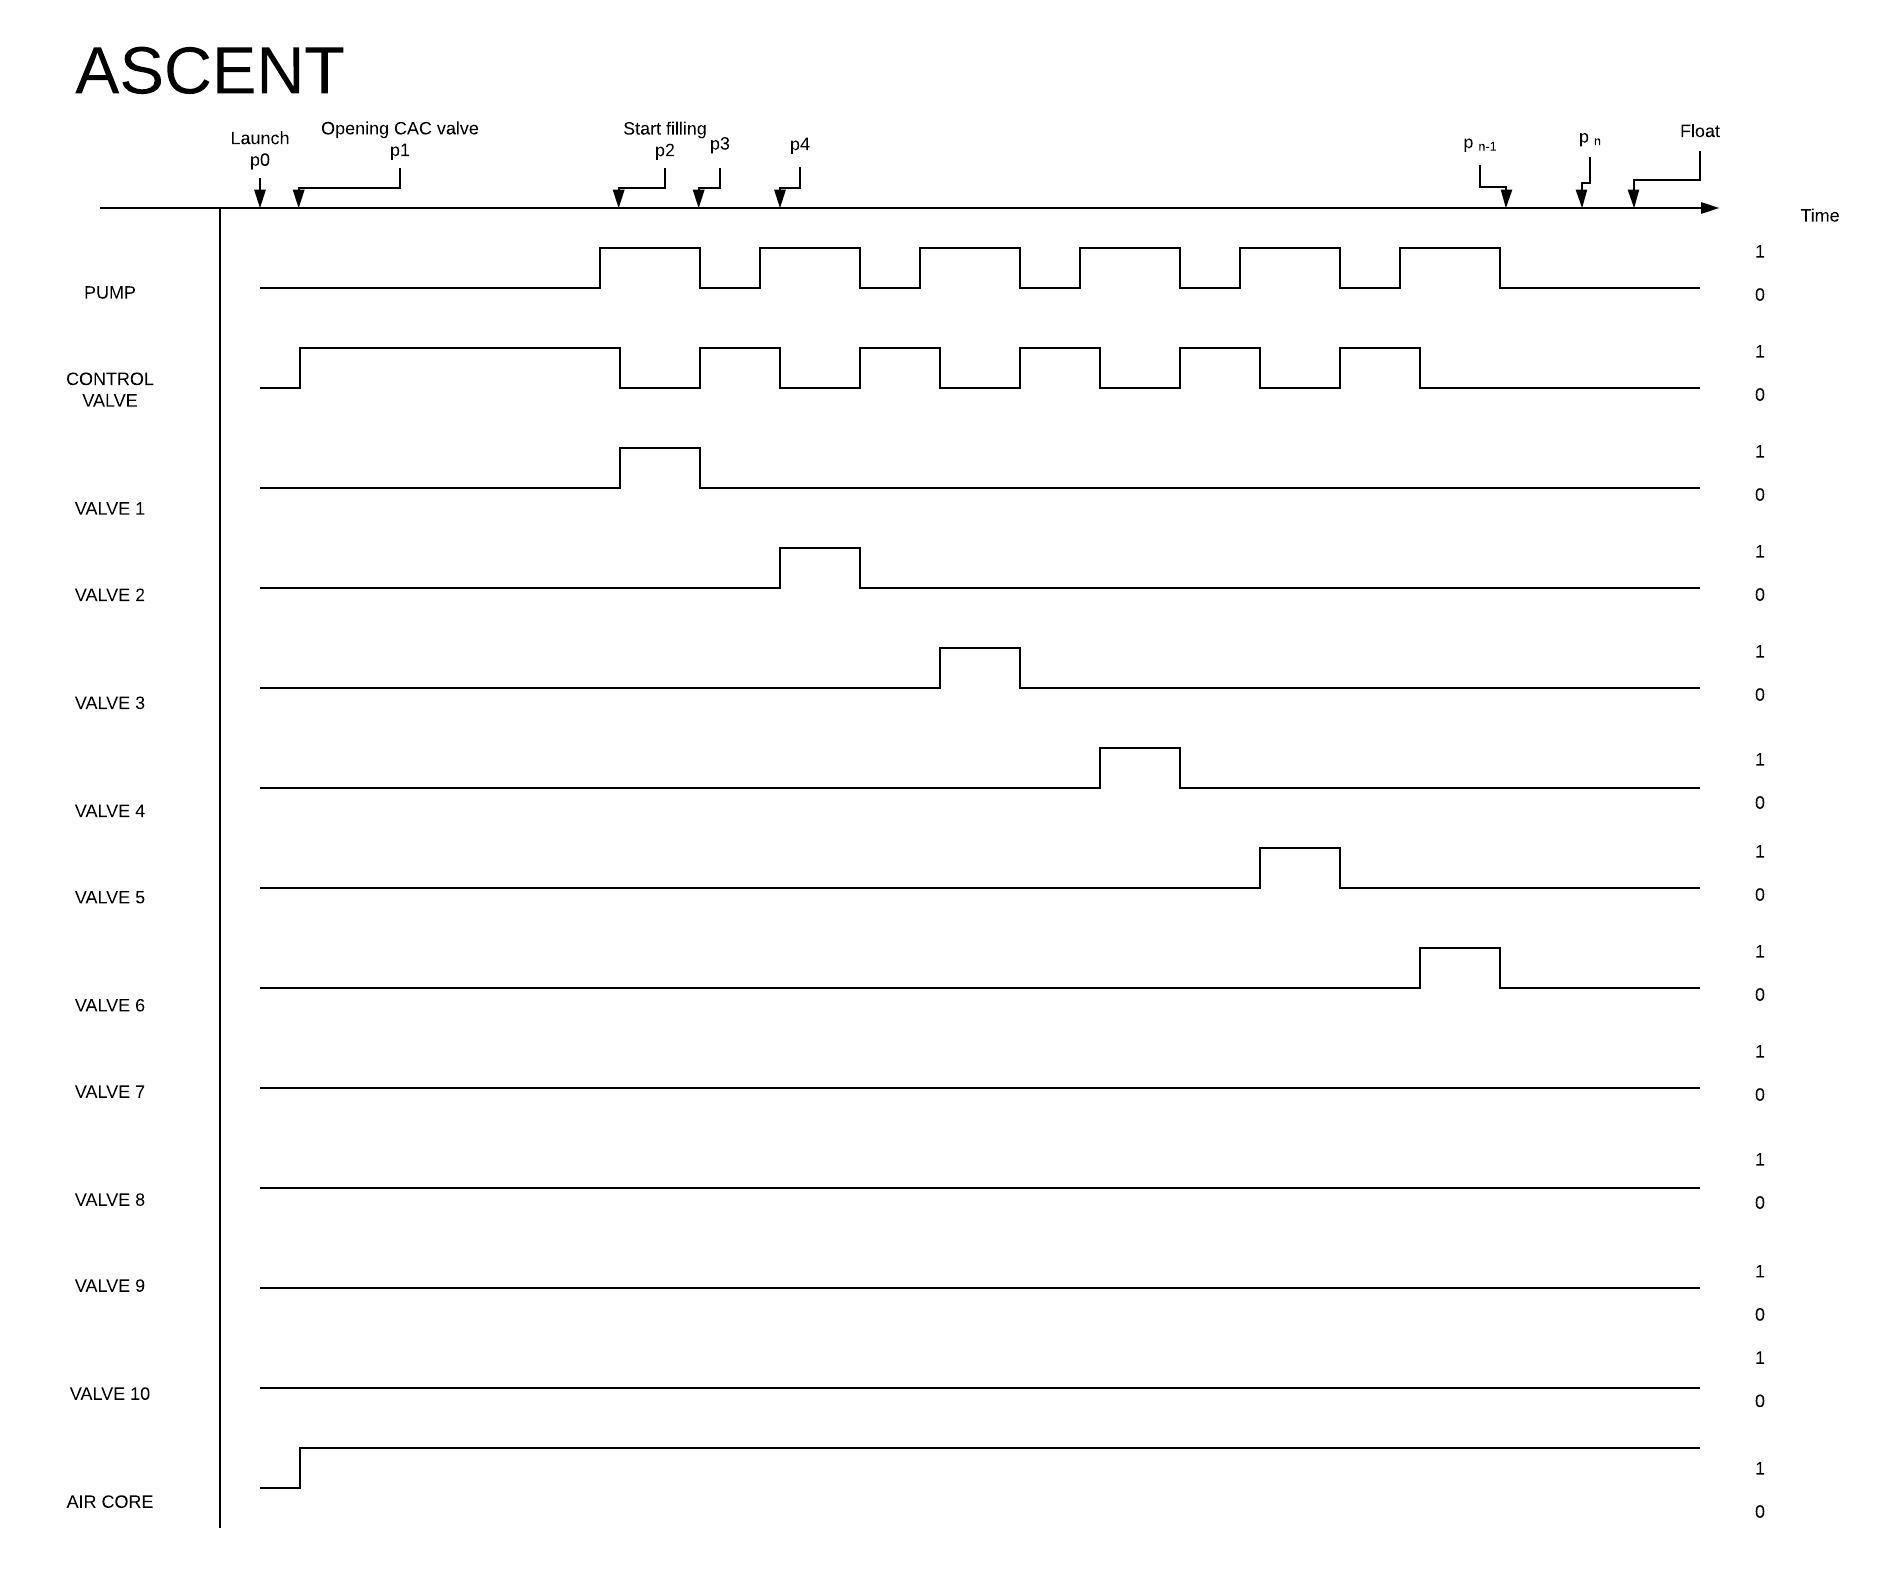
\includegraphics[width=1\linewidth]{4-experiment-design/img/ascent-phase.jpeg}
    \end{align*}
    \caption{The Emptying and Sampling Sequence-Ascent Phase.}
    \label{fig:ascent}
\end{figure}

\begin{figure}[H]
    \begin{align*}
        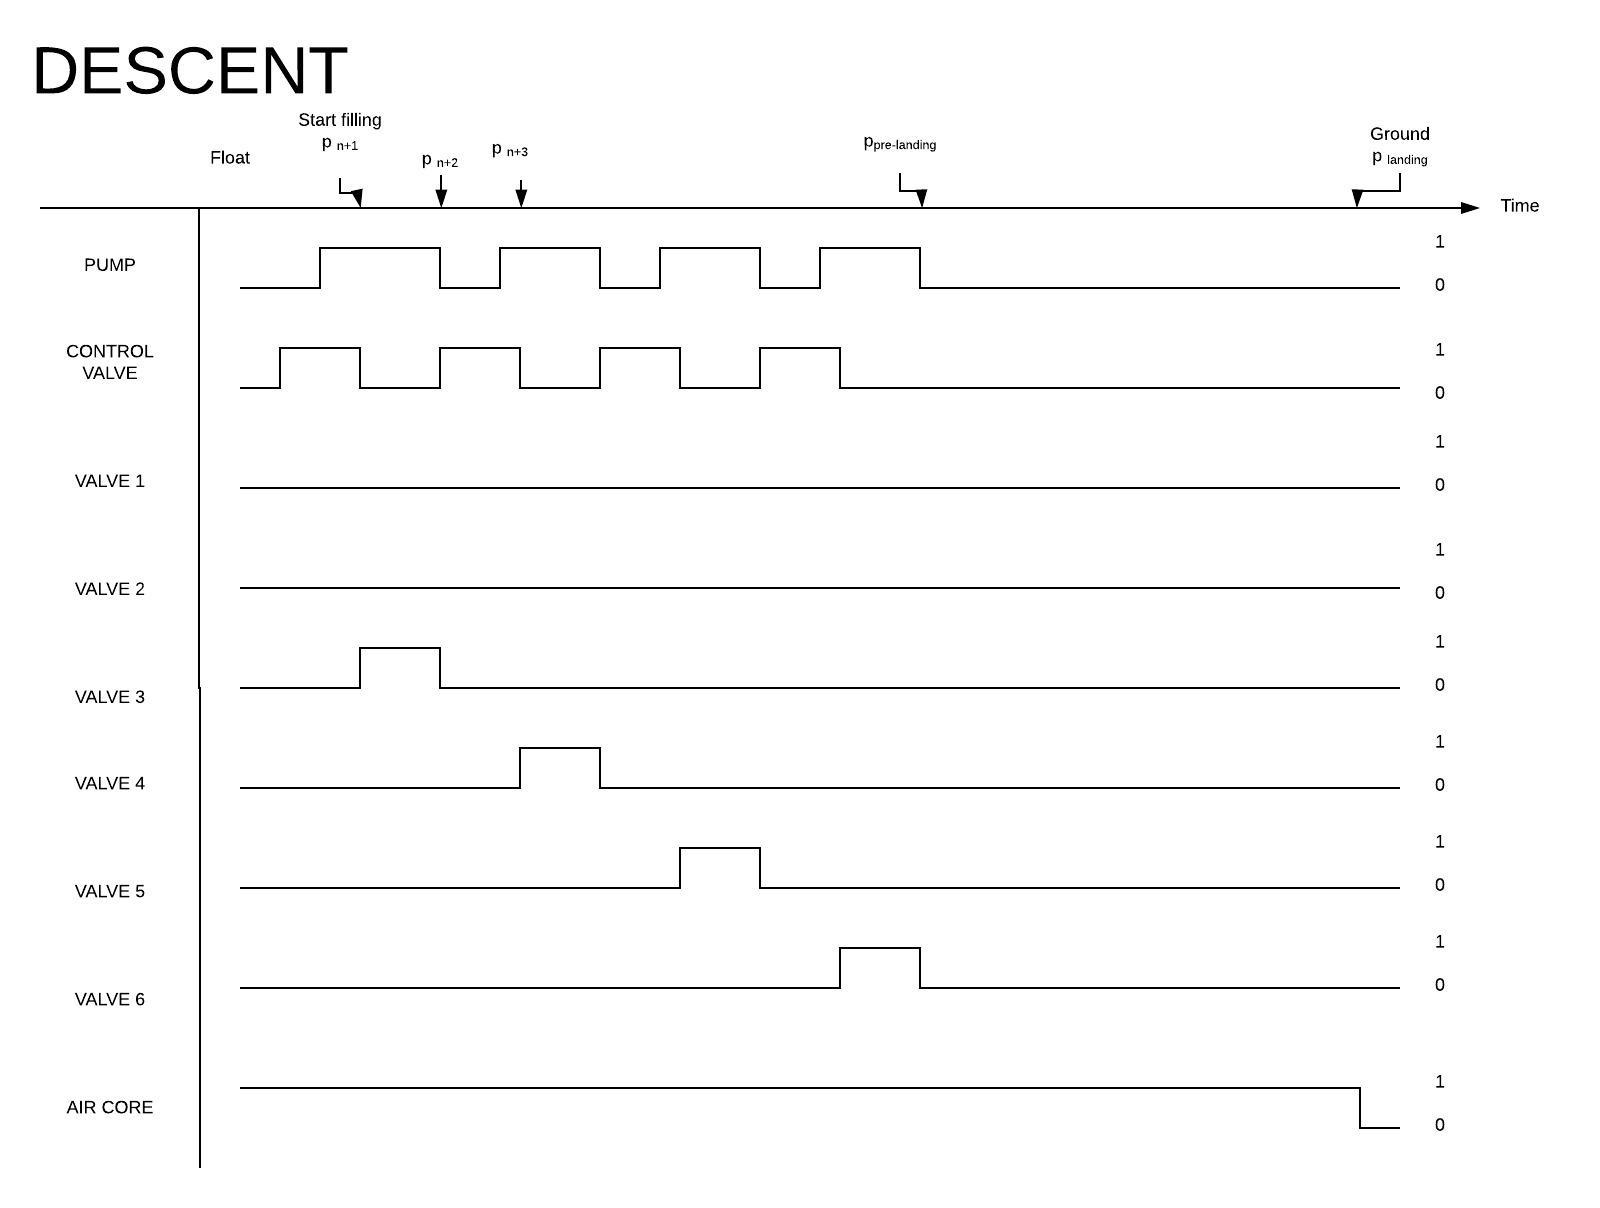
\includegraphics[width=1\linewidth]{4-experiment-design/img/descent-phase.jpeg}
    \end{align*}
    \caption{The Emptying and Sampling Sequence-Descent Phase.\label{fig:descent}}
\end{figure}

In the diagrams, 0 denotes closed/off and 1 denotes opened/on. The horizontal axis denotes the different pressure levels throughout the flight, with p$_0$ being the sea level pressure and p$_8$ being the pressure during Float Phase.

The ambient pressure dependent timeline of the experiment is as follow:

\textbf{Ascent Phase:}\\
$p_0$ – $p_1$
\begin{itemize}
    \item CAC valve shall be closed.
    \item AAC valves shall be closed.
    \end{itemize}
$p_1$ – $p_2$
\begin{itemize}
    \item CAC valve shall be opened.
    \item CAC tube shall start flushing.
    \end{itemize}
    
$p_2$ – $p_3$
\begin{itemize}
    \item AAC flushing valve shall be opened, allowing for the system to flush.
    \item CAC valve remains open.
    \end{itemize}
$p_3$ – $p_4$
\begin{itemize}
    \item AAC flushing valve shall be closed.
    \item Valve 1 shall be opened, allowing for air to enter the first bag.
    \item CAC valve remains open.
    \end{itemize}
$p_4$ – $p_5$
\begin{itemize}
    \item Valve 1 shall be closed.
    \item AAC flushing valve shall be closed.
    \item CAC valve remains open.
    \end{itemize}
$p_5$ - $p_6$    
 \begin{itemize}
    \item AAC flushing valve shall be opened, allowing the system to flush. 
    \item CAC valve remains open.
    \end{itemize}
$p_6$ - $p_7$
\begin{itemize}
    \item AAC flushing valve shall be closed.
    \item Valve 2 shall be opened, allowing for air to enter the second bag.
    \item CAC valve remains open.
    \end{itemize}
$p_7$ - $p_8$
\begin{itemize}
    \item Valve 2 shall be closed.
    \item AAC flushing valve shall be closed.
    \item CAC shall finish flushing.
    \end{itemize}    
    



\textbf{\\Float Phase:}\\
No action is taken other than continued telemetry.
 
\textbf{Descent Phase:}
 
$p_9$ – $p_{10}$
\begin{itemize}
    \item CAC shall start sampling. 
    \item AAC valves shall be closed.
\end{itemize}

$p_{10}$ – $p_{11}$
\begin{itemize}
    \item AAC flushing valve shall be opened allowing the system to flush.
    \item CAC valve remains open. 
\end{itemize}
 
  
$p_{11}$ – $p_{12}$
\begin{itemize}
    \item AAC flushing valve shall be closed.
    \item Valve 3 shall be opened, allowing for air to enter the third bag.
    \item CAC valve remains open. 
\end{itemize}

$p_{12}$ – $p_{13}$
\begin{itemize}
    \item Valve 3 shall be closed.
    \item AAC flushing valve shall be closed.
    \item CAC valve remains open.
\end{itemize}

$p_{13}$ – $p_{14}$
\begin{itemize}
    \item AAC flushing valve shall be opened allowing the system to flush.
    \item CAC valve remains open.
\end{itemize}

$p_{14}$ – $p_{15}$
\begin{itemize}
    \item AAC flushing valve shall be closed.
    \item Valve 4 shall be opened, allowing for air to enter the fourth bag.
    \item CAC valve remains open.
\end{itemize}

$p_{15}$ – $p_{16}$
\begin{itemize}
    \item Valve 4 shall be closed.
    \item AAC flushing valve shall be closed.
    \item CAC valve remains open.
\end{itemize}

$p_{16}$ – $p_{17}$
\begin{itemize}
    \item AAC flushing valve shall be opened, allowing the system to flush. 
    \item CAC remains open.
  \end{itemize}

$p_{17}$ – $p_{18}$
\begin{itemize}
    \item AAC flushing valve shall be closed.
    \item Valve 5 shall be opened, allowing for air to enter the fifth bag. 
    \item CAC valve remains open.
\end{itemize}

$p_{18}$ – $p_{19}$
\begin{itemize}
    \item Valve 5 shall be closed.
    \item AAC flushing valve shall be closed.
    \item CAC valve remains open.
\end{itemize}

$p_{19}$ – $p_{20}$
\begin{itemize}
     \item AAC flushing valve shall be opened, allowing the system to flush. 
    \item CAC remains open.
   \end{itemize}

$p_{20}$ – $p_{21}$
\begin{itemize}
    \item AAC flushing valve shall be closed.
    \item Valve 6 shall be opened, allowing for air to enter the sixth bag.
\end{itemize}

$p_{pre-landing}$ 
\begin{itemize}
    \item Valve 6 shall be closed.
    \item AAC flushing valve shall be closed.
    \item CAC valve shall be opened.
\end{itemize}

$p_{0-landing}$
\begin{itemize}
    \item CAC valve shall be closed.
\end{itemize}


Note: The AAC system's air pump is only on during sampling into the air sampling bags and flushing of the system.


\raggedbottom